Der zweite Teilversuch befasst sich mit der Lichtquelle eines handelsüblichen LCD-Beamer, einer sogenannten Quecksilberdampflampe. Sie liefert durch Gasentladungen einen starken, gebündelten und möglichst gleichmäßig spektral verteilten Lichtstrahl, welcher zur Projektion der Bilder des Beamers verwendet wird. Das Spektrum dieser Lampe beeinflusst maßgeblich die Farben, welche dem später betrachteten LCD-Beamer zur Verfügung stehen, und ist somit in Kombination mit den dichroitischen Spiegeln wichtiger Teil der Farbwiedergabe selbst.

In diesem Versuch soll das Spektrum und der Lichtstrom $\Phi_{e,\lambda}$ einer solchen Quecksilberdampflampe mithilfe einer Ulbrichtkugel bestimmt werden. Diese ist eine von innen streuend reflektierende Kugel, welche die Bestimmung des absoluten Lichstroms der Lampe anhand einer einzelnen Punktmessung ermöglicht. Wichtig ist hierbei auch eine korrekte Vermessung eines Referenz- und Absorptionsspektrums, um aus der Punktmessung der Lampe auf den realen Lichtstrom schließen zu können.

\subsubsection{Versuchsaufbau}

Der Versuchsaufbau besteht aus einer bereits aufgebauten Ulbrichtkugel inklusive Spektrometer, der Quecksilberdampflampe und einer Absorptionskorrekturlampe. Um die Lampen betreiben zu können steht eine Spannungsquelle zur Verfügung. Das Spektrometer wird von einem Computer aus bedient, von welchem die gemessenen Spektren gespeichert werden können.

\subsubsection{Versuchsdurchführung}

Die Kalibrationsdaten der im Versuch verwendeten Ulbrichtkugel sind bekannt. Für andere, nicht bereits kalibierte Kugeln muss vor dem Versuch noch das Referenzspektrum $D_{\lambda,ref}$ einer bekannten Referenzlampe (mit bekanntem $\Phi_{e\lambda,ref}$), sowie das Spektrum der Absorptionskorrekturlampe $K_{\lambda,ref}$ (ohne eingebaute Quecksilberdampflampe) bestimmt werden.

Die Messung des Spektrums der Quecksilberdampflampe ($D_\lambda(\lambda)$) erfolgt in den folgenden Schritten:

\begin{itemize}
\item Das Spektrum der Absorptionskorrekturlampe mit eingebauter Quecksilberdampflampe, $K_\lambda$, wird gemessen. Die Absorptionskorrekturlampe wird hierfür eingeschaltet, die Dampflampe bleibt aus. Das Spektrum wird am Computer gespeichert.
\item Das Spektrum der eingeschalteten Quecksilberdampflampe, $D_\lambda$, wird gemessen. Hierfür muss die Lampe einige Minuten vorwärmen, um sich zu stabilisieren. Der Lüfter der Lampe muss hierfür laufen, da sich die Lampe ansonsten zu stark erhitzt. Das Spektrum wird am Computer abgespeichert.
\end{itemize}
Die gemessenen Spektren sind in Grafiken \ref{V2_AKL} und \ref{V2_QDL} dargestellt.

\subsubsection{Auswertung}

\label{V2_AUSW}

\begin{figure}[h]
	\centering
	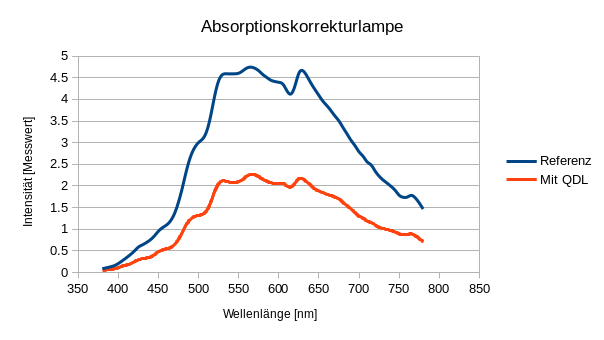
\includegraphics[scale=0.8]{Images/V2_AKL.png}
	\caption{Gemessenes Spektrum der Absorptionskorrekturlampe im Vergleich zum Referenzspektrum}
	\label{V2_AKL}
\end{figure}

Zuerst wird das Absorptionsspektrum der Absorptionskorrekturlampe, sichtbar in Abbildung \ref{V2_AKL}, mit dem bereitgestellten Referenzwert verglichen. Deutlich zu sehen ist, dass der gemessene Wert um einen Faktor von etwa 2 kleiner ist als der Referenzwert. Das Gehäuse der Quecksilberdampflampe absorbiert also etwa die Hälfte des Lichtes, gleichmäßig über das Spektrum verteilt.
Zur Berechnung der Korrekturfaktoren muss lediglich das Referenzspektrum durch das gemessene Spektrum dividiert werden.
\begin{equation}
\frac{K_{\lambda,ref}(\lambda)}{K_{\lambda}(\lambda)}
\end{equation}
In Abbildung \ref{V2_KOR} ist deutlich ein einheitlicher Faktor von ca. 2 erkennbar, welcher nur leicht mit der Wellenlänge schwankt. Dies ist vom schwarzen Plastikgehäuse zu erwarten.

\begin{figure}[h]
	\centering
	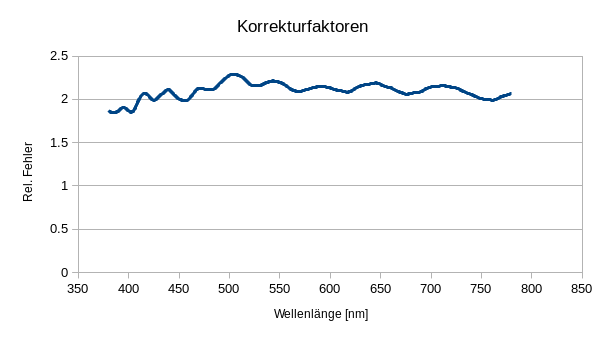
\includegraphics[scale=0.7]{Images/V2_Korr.png}
	\caption{Berechnete Wellenlängenabhängige Korrekturfaktoren}
	\label{V2_KOR}
\end{figure}

\begin{figure}[h]
	\centering
	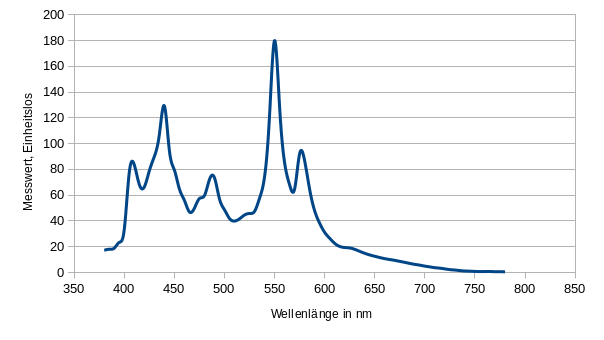
\includegraphics[scale=0.7]{Images/V2_Dampflampe.png}
	\caption{Messwerte des Quecksilberdampflampenspektrums}
	\label{V2_QDL}
\end{figure}

In Abbildung \ref{V2_QDL} ist nun das gemessene Spektrum der Quecksilberdampflampe zu sehen. Erkennbar ist dass über den gesamten sichtbaren Wellenlängenbereich (400nm bis 600nm) Licht abgestrahlt wird. Dies passiert jedoch sehr Wellenlängenabhängig, mit deutlichen Peaks um 400nm, 440nm, 480nm, 550nm und 570nm. Sie entstehen durch die Arbeitsweise der Dampflampe, da die angeregten Elektronen nur bestimmte Wellenlängen aussenden können.

Der Lichtstrom der Dampflampe, $\Phi_{e,\lambda}(\lambda)$, kann nun bestimmt werden. Hierfür werden die Messwerte zuerst mit den berechneten Absorptionskorrekturfaktoren multipliziert, und anschließend mithilfe der bereitgestellten Referenzwerte in den absoluten spektralen Lichtstrom umgerechnet. Es gilt anhand von [\cite[Seite 22]{AML_SKRIPT}] folgende Gleichung. Der berechnete Lichtstrom ist in Abbildung \ref{V2_STROM} dargestellt.

\begin{equation}
\Phi_{e\lambda}(\lambda) = \Phi_{e\lambda,ref}(\lambda)\cdot \frac{D_{\lambda}(\lambda)}{D_{\lambda,ref}(\lambda)} \cdot \underbrace{\frac{K_{\lambda,ref}(\lambda)}{K_{\lambda}(\lambda)}}_{\mbox{Korrekturfaktor}}
\end{equation}

\begin{figure}[h]
	\centering
	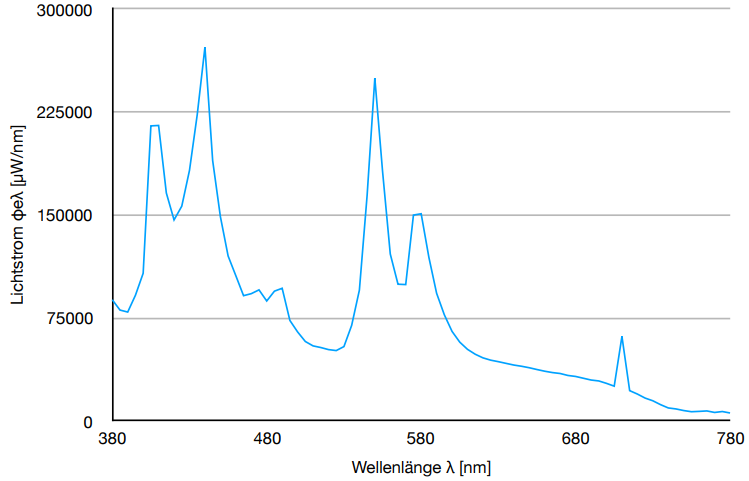
\includegraphics[scale=0.4]{Images/V2_Lichtstrom.png}
	\caption{Berechneter spektraler Lichtstrom der Quecksilberdampflampe}
	\label{V2_STROM}
\end{figure}